\documentclass[../../../../main.tex]{subfiles}

\begin{document}

\section*{京大理科数学 1972 表紙・配点・概略}

\begin{itemize}
    \item 所要時間: 70分 / 150分
\end{itemize}

\subsection*{難易度・分野一覧}
\begin{enumerate}
    \item 論理 (難易度: C, 計算: A, 思考: C)
    \item 極限 (難易度: A, 計算: A, 思考: A)
    \item 多変数 (難易度: B, 計算: B, 思考: B)
    \item 図形 (難易度: C, 計算: B, 思考: C)
    \item 多変数 (難易度: A, 計算: A, 思考: A)
    \item 確率 (難易度: A, 計算: A, 思考: A)
\end{enumerate}

\subsection*{各問のメモ・解答概要}
\begin{enumerate}
    \item 論理: 帰納法により証明
    \item 極限: $-\frac{3}{2}\log 3$
    \item 多変数: $x, y, z$ のうち少なくとも1つは $a$ である
    \item 図形: (手書き解答なし)
    \item 多変数: $u = \frac{1}{ab} t$
    \item 確率: $2E$
\end{enumerate}

\newpage

\section*{第1問}

\noindent
[\textbf{解}] ベクトルの2つの公理を①, ②とする. すなわち,
\[
\vec{A} + \vec{B} = \vec{B} + \vec{A} \quad \cdots \text{①}
\]
\[
(\vec{A} + \vec{B}) + \vec{C} = \vec{A} + (\vec{B} + \vec{C}) \quad \cdots \text{②}
\]
以下, $\vec{S_n} = \sum_{k=1}^n \vec{A_k}$, $\vec{T_n} = \sum_{k=1}^n \vec{B_k}$ とする. $\vec{S_n} = \vec{T_n} \quad \cdots$ ③ を帰納的に示す.

\paragraph{[補題1]}
任意のベクトル $\vec{a_1}, \dots, \vec{a_n}$ に対し ($n \ge 2$)
\[
\vec{a_1} + \dots + \vec{a_n} = \vec{a_2} + \vec{a_3} + \dots + \vec{a_n} + \vec{a_1} \quad \cdots \star
\]

(証) 帰納法による. $n=2$ の時は $\star$ は ①に他ならない. $n=k$ での成立を仮定すると, $n=k+1$ の時
\begin{align*}
\vec{a_1} + \dots + \vec{a_{k+1}} &= \vec{a_1} + \dots + \vec{a_{k-1}} + (\vec{a_k} + \vec{a_{k+1}}) \quad (\because \text{②}) \\
&= \vec{a_2} + \dots + (\vec{a_k} + \vec{a_{k+1}}) + \vec{a_1} \quad (\because \text{仮定}) \\
&= \vec{a_2} + \dots + \vec{a_k} + \vec{a_{k+1}} + \vec{a_1} \quad (\because \text{②})
\end{align*}
ゆえに $n=k+1$ でも $\star$ は成立.
以上から $\star$ は示された. \hfill 終

\bigskip
まず, $n=1$ の時. ③ $\iff \vec{A_1} = \vec{B_1}$ でこれは定義から成立する. そこで $i \in \mathbb{N}$ に対し, $n \le i$ での③の成立を仮定する. $n=i+1$ の時, $k=0, 1, \dots, i$ に対して,
\[
\vec{A_{i+1}} = \vec{B_{k+1}}
\]
なる $k$ があることに注意する.

\begin{enumerate}
    \item[$1^\circ$] $k=i$ の時
    \begin{align*}
    \vec{T_{i+1}} &= \vec{T_i} + \vec{B_{i+1}} \\
    &= \vec{S_i} + \vec{A_{i+1}} \quad (\because \text{仮定}, \vec{A_{i+1}} = \vec{B_{i+1}}) \\
    &= \vec{S_{i+1}}
    \end{align*}
    となり, $n=i+1$ でも ③は成立.

    \item[$2^\circ$] $k \ne i$ の時
    \begin{align*}
    \vec{T_{i+1}} &= \vec{B_1} + \dots + \vec{B_k} + \vec{B_{k+1}} + \vec{B_{k+2}} + \dots + \vec{B_{i+1}} \\
    &= \vec{B_{k+1}} + \vec{B_1} + \dots + \vec{B_k} + \vec{B_{k+2}} + \dots + \vec{B_{i+1}} \quad (\because \text{仮定}) \\
    &= \vec{B_1} + \dots + \vec{B_k} + \vec{B_{k+2}} + \dots + \vec{B_{i+1}} + \vec{B_{k+1}} \quad (\because \text{補題1}) \\
    &= \vec{S_{i+1}} \quad (\because 1^\circ \text{に帰着})
    \end{align*}
\end{enumerate}

以上 $1^\circ, 2^\circ$ から, $n=i+1$ でも ③は成立する. ゆえに③は示された. \hfill 終

\newpage

\section*{第2問}

\noindent
[\textbf{解}]
\begin{align*}
F(x) &= \int_2^x \frac{1}{2}\left( \frac{1}{t+1} - \frac{3}{t+3} \right) dt \\
&= \frac{1}{2} \left[ \log(t+1) - 3\log(t+3) \right]_2^x \\
&= \frac{1}{2} \left( \log(x+1) - 3\log(x+3) + 3\log 3 \right)
\end{align*}
だから
\begin{align*}
F(x) - \log x &= -\frac{3}{2}\log 3 + \frac{3}{2}\log(x+3) - \frac{1}{2}\log(x+1) - \log x \\
&= -\frac{3}{2}\log 3 + \frac{1}{2}\log \frac{(x+3)^3}{(x+1)x^2} \\
&= -\frac{3}{2}\log 3 + \frac{1}{2}\log \frac{(1 + \frac{3}{x})^3}{1 + \frac{1}{x}} \longrightarrow -\frac{3}{2}\log 3 \quad (x \to \infty)
\end{align*}
$(\because \log x \text{ は連続})$

\newpage

\section*{第3問}

\noindent
[\textbf{解}] $x' = x-a, y' = y-a, z' = z-a$ とおく. 手をくわえて
\[
\begin{cases}
x' + y' + z' = -2a \quad \cdots \text{①} \\
(x'+a)^3 + (y'+a)^3 + (z'+a)^3 = a^3 \quad \cdots \text{②}
\end{cases}
\]
ここで, $P = x'^2 + y'^2 + z'^2$, $Q = y'z' + z'x' + x'y'$ とおく. ①より $a = -\frac{1}{2}(x'+y'+z')$ だから, ②に代入
\[
r + \frac{3}{2} P (x'+y'+z') + \frac{3}{4} (x'+y'+z')^2 - \frac{1}{4} (x'+y'+z')^3 = 0
\]
\[
(x'+y'+z')(P-Q) + 3x'y'z' + \frac{1}{2}(x'+y'+z') [ (x'+y'+z')^2 - 3P ] = 0
\]
\[
(x'+y'+z')(P-Q) + 3x'y'z' + (x'+y'+z')(P + 2Q - 3P) = 0
\]
\[
x'y'z' = 0
\]
よって $x', y', z'$ のうち少なくとも1つは 0, つまり $x, y, z$ のうち少なくとも1つは $a$ である.

\bigskip
\noindent
[\textbf{解2}] (直接示す)
\[
x^3 + y^3 + z^3 = (x+y+z)^3
\]
展開する
\[
3x^2 y + 3x^2 z + 3y^2 x + 3y^2 z + 3z^2 x + 3z^2 y + 6xyz = 0
\]
\[
(y+z)(z+x)(x+y) = 0
\]
よって OK \hfill 終

\newpage

\section*{第5問}

\noindent
[\textbf{解}] $X = \frac{x}{a}, Y = \frac{y}{b}$ なる変換をほどこす.

$P$ は $P'(\cos u, b \sin u)$ に, 楕円は $X^2 + Y^2 = 1$ にうつり, $OP$ のはいった部分は下図斜線部(この面積 $S'$ とする)にうつる. 変換の定義から
\[
S = S' ab \quad \cdots \text{①}
\]
であり,
\[
S' = \frac{1}{2} u
\]
だから①に代入して
\[
S = \frac{1}{2} ab u
\]
$\frac{dS}{dt} = 1$ より
\[
\frac{dS}{dt} = \frac{1}{2} ab \frac{du}{dt} = 1
\]
\[
\therefore \frac{du}{dt} = \frac{1}{ab}
\]
\[
du = \frac{1}{ab} dt
\]
積分して
\[
u = \frac{1}{ab} t + C \quad (C \text{:定数})
\]
$t=0$ で $u=0$ より $C=0$ だから, \underline{$u = \frac{1}{ab} t$} である.

\begin{center}
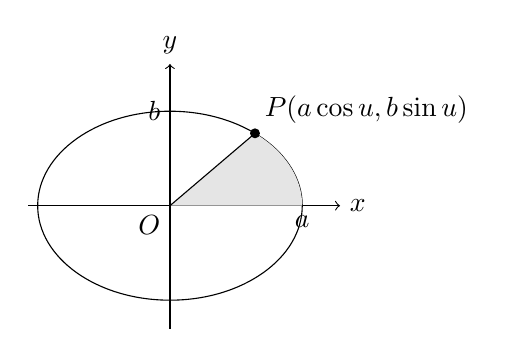
\begin{tikzpicture}[scale=1.2]
    \draw[->] (-1.5,0) -- (1.8,0) node[right] {$x$};
    \draw[->] (0,-1.3) -- (0,1.5) node[above] {$y$};
    \node[below left] at (0,0) {$O$};
    \draw (0,0) ellipse (1.4cm and 1.0cm);
    \fill[gray!20] (0,0) -- (1.4,0) arc (0:50:1.4cm and 1.0cm) -- cycle;
    \draw (0,0) -- (50:1.4cm and 1.0cm) node[above right] {$P(a\cos u, b\sin u)$};
    \fill (50:1.4cm and 1.0cm) circle (1.5pt);
    \node[below] at (1.4,0) {$a$};
    \node[left] at (0,1.0) {$b$};
\end{tikzpicture}
\hspace{1cm}
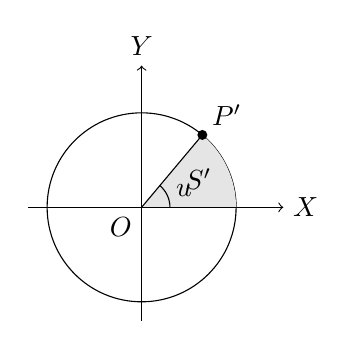
\begin{tikzpicture}[scale=1.2]
    \draw[->] (-1.2,0) -- (1.5,0) node[right] {$X$};
    \draw[->] (0,-1.2) -- (0,1.5) node[above] {$Y$};
    \node[below left] at (0,0) {$O$};
    \draw (0,0) circle (1.0cm);
    \fill[gray!20] (0,0) -- (1.0,0) arc (0:50:1.0cm) -- cycle;
    \draw (0,0) -- (1.0,0);
    \draw (0,0) -- (50:1.0cm) node[above right] {$P'$};
    \fill (50:1.0cm) circle (1.5pt);
    \draw (0.3,0) arc (0:50:0.3cm);
    \node at (0.45,0.18) {$u$};
    \node at (0.6,0.3) {$S'$};
\end{tikzpicture}
\end{center}

\newpage

\section*{第6問}

\noindent
[\textbf{解}] まず, $A = \sum_{k=1}^n a_k$ とおいて, $E = \frac{1}{n} A$ である $\cdots$ ①. 次に $F$ について, 取り出した2枚を区別して考える. 1枚目の数 $X$, 2枚目の数 $Y$ とおくと
\[
F = E(X+Y) = E(X) + E(Y)
\]
である. 明らかに $E(X) = E \cdots$ ② である. 以下 $E(Y)$ について
\[
E(Y) = \frac{1}{n} \cdot \left( \sum_{k=1}^n \frac{A - a_k}{n-1} \right) = \frac{1}{n} \cdot \frac{n-1}{n-1} A = \frac{1}{n} A \quad \cdots \text{③}
\]
①, ②, ③から
\[
F = \frac{1}{n} A + \frac{1}{n} A = 2E \quad \text{答}
\]

\end{document}
